\section{Experiments}
\label{sec:exps}


\begin{figure}[t]

\centering
\begin{subfigure}{0.20\textwidth}
    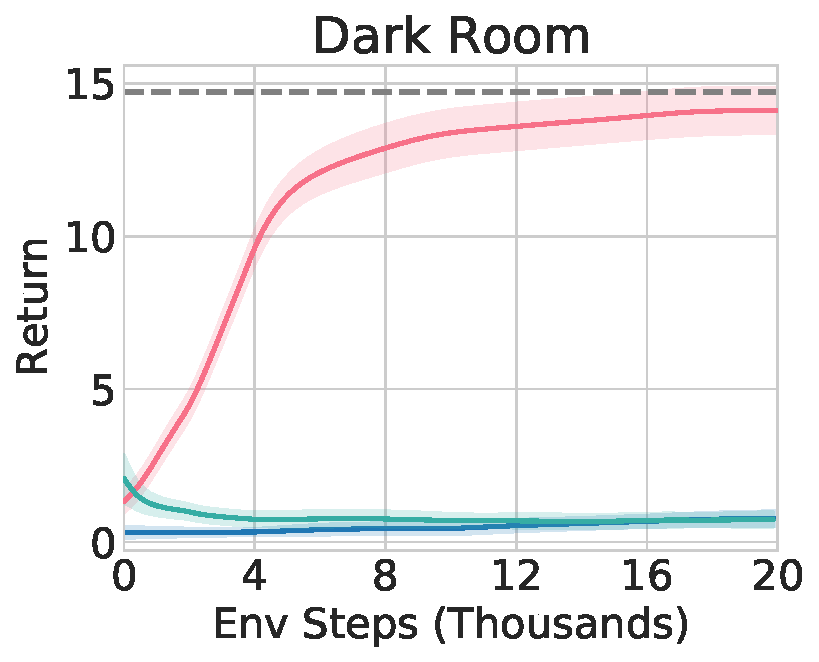
\includegraphics[width=\textwidth]{assets/images/9x9_1g_dense_main.pdf}
 
\end{subfigure}
\hfill
\begin{subfigure}{0.20\textwidth}
    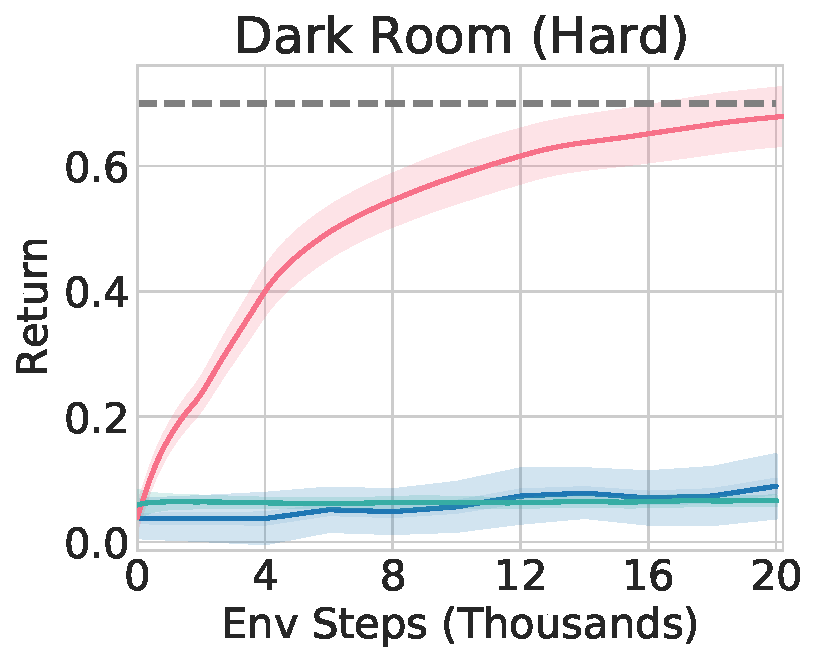
\includegraphics[width=\textwidth]{assets/images/dark_room_hard_main.pdf}
 
\end{subfigure}
\hfill
\begin{subfigure}{0.20\textwidth}
    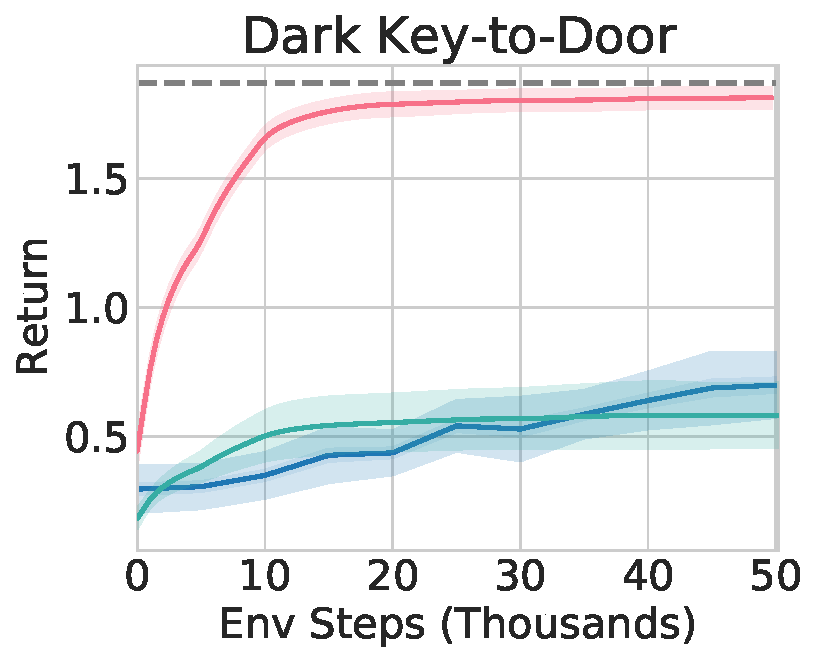
\includegraphics[width=\textwidth]{assets/images/dark_key_door_main.pdf}
\end{subfigure}
\hfill
\begin{subfigure}{0.216\textwidth}
    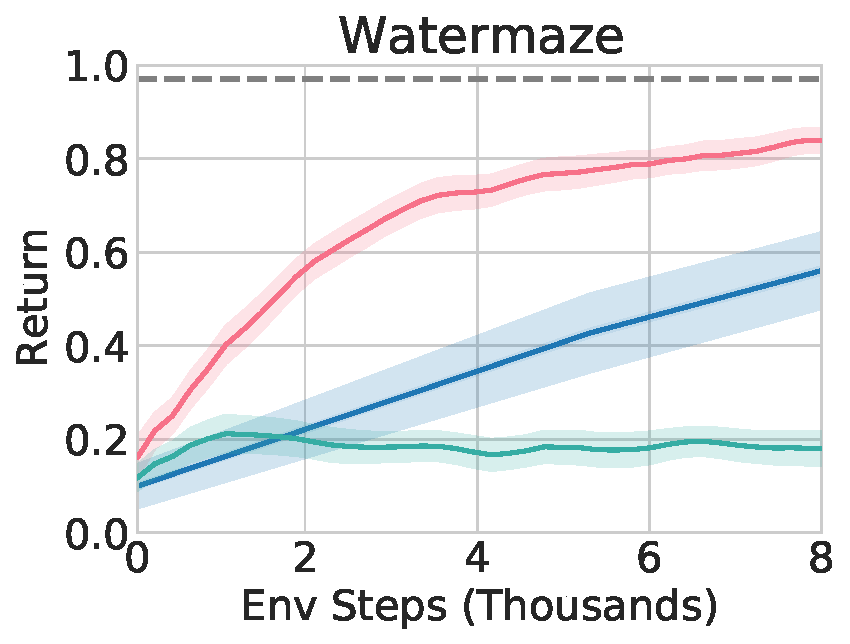
\includegraphics[width=\textwidth]{assets/images/watermaze_main_160_epi.pdf}

\end{subfigure}
\hfill
\begin{subfigure}{0.14\textwidth}
    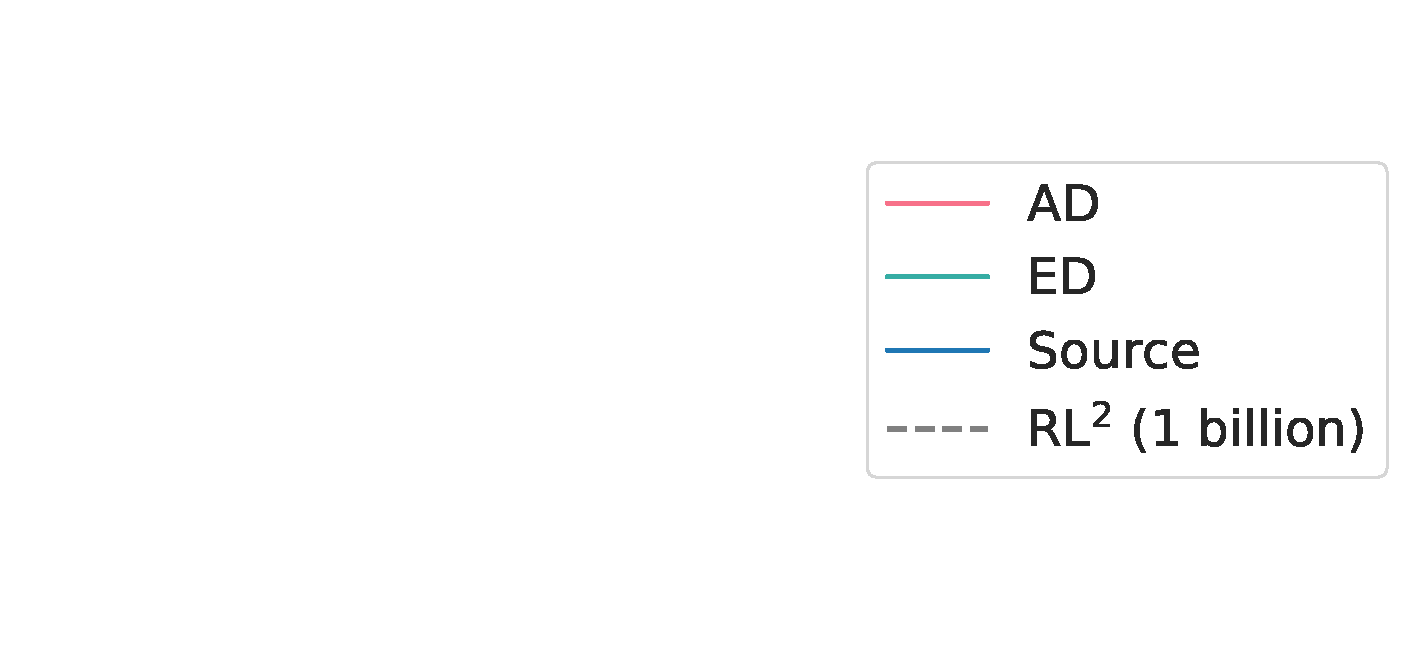
\includegraphics[width=\textwidth]{assets/images/legend_main.pdf}

\end{subfigure}
\caption{\small {\it Main results:} we evaluate \namenospace, $\text{RL}^2$, ED, and the source algorithm on environments that require memory and exploration. In these environments, an agent must reach a goal location that can only be inferred through a binary reward. \name is consistently able to in-context reinforcement learn across all environments and is  more data-efficient than the A3C (``Dark'' environments)~\citep{mnih16a3c} or DQN (Watermaze)~\citep{mnih2013dqn} source algorithm it distilled. We report the mean return $\pm$ 1 standard deviation over 5 training seeds with 20 test seeds each. }
\label{fig:main_exps}
\vspace{-4mm}
\end{figure}



The main research question of this work is whether an in-weights RL algorithm can be amortized into an in-context one via \fullnamenospace.
The in-context RL algorithm should behave in a similar way as the in-weights one and exhibit exploration, credit assignment, and generalization capabilities. We begin our analysis in a clean and simple experimental setting where all three properties are required to solve the task - the Adversarial Bandit described in Sec.~\ref{sec:experimental-setup}.

To generate the source data, we sample a set of training tasks $\{ \mathcal M_j\}_{j=1}^N$, run the Upper Confidence Bound algorithm~\citep{lai86ucb}, and save its learning histories. We then train a transformer to predict actions as described in Alg.~\ref{alg:ad_full}. We evaluate \namenospace, ED, and $\text{RL}^2$ and normalize their scores relative to UCB and a random policy ${(r - r_{rand.})}/{ (r_{UCB} - r_{rand.})}$. The results are shown in Fig.~\ref{fig:bandit}. We find that both \name and RL$^2$ can reliably in-context learn tasks sampled from the training distribution while ED cannot, though ED does do better than random guessing when evaluated in-distribution. However, \name can also in-context learn to solve out of distribution tasks whereas the other methods cannot. This experiment shows that \name can explore the bandit arms, can assign credit by exploiting an arm once reached, and can generalize well out of distribution nearly as well as UCB. We now move beyond the bandit setting and investigate similar research questions in more challenging RL environments and present our results as answers to a series of research questions. 


\vspace{-2mm}
\paragraph{Does Algorithm Distillation exhibit in-context reinforcement learning?}

To answer this question, we first generate source data for \fullnamenospace.
In the Dark Room and Dark Key-to-Door environments we collect $2000$ learning histories with an Asynchronous Advantage Actor-Critic (A3C)~\citep{mnih16a3c} with $100$ actors, while in DMLab Watermaze we collect $4000$ learning histories with a distributed DQN with 16 parallel actors (see Appendix~\ref{app:source} for asymptotic learning curves of the source algorithm and Appendix~\ref{app:rl_hypers} for hyperparameters). Shown in Fig.~\ref{fig:main_exps}, \name in-context reinforcement learns in all of the environments. In contrast, ED fails to explore and learn in-context in most settings. We use RL$^2$ trained for 1 billion environment steps as a proxy for the upper bound of performance for a meta-RL method. Despite learning to reinforcement learn from offline data, \name matches asymptotic RL$^2$ on the Dark environments and approaches it (within $13\%$) on Watermaze.

\noindent{\it Credit-assignment:} In Dark Room, the agent receives $r=1$ each time it visits the goal location. Even though \name is trained to condition only on single timestep reward and not episodic return tokens, it is still able to maximize the reward, which suggests that \name has learned to do credit assignment.

\noindent{\it Exploration:} Dark Room (Hard) tests the agents exploration capability. Since the reward is sparse ($r=1$ exactly once), most of the learning history has reward values of $r=0$. Nevertheless, \name infers the goal from previous episodes in its context which means it has learned to explore and exploit.

\noindent{\it Generalization:} Dark Key-to-Door tests in-distribution generalization with a combinatorial task space. While the environment has a total of $\sim6.5$k tasks, less than $2$k were seen during training. During evaluation, \name both generalizes and achieves near-optimal performance on mostly unseen tasks.


\begin{figure}[h]

\centering
  \hspace*{\fill}%
\begin{subfigure}{0.4\textwidth}
    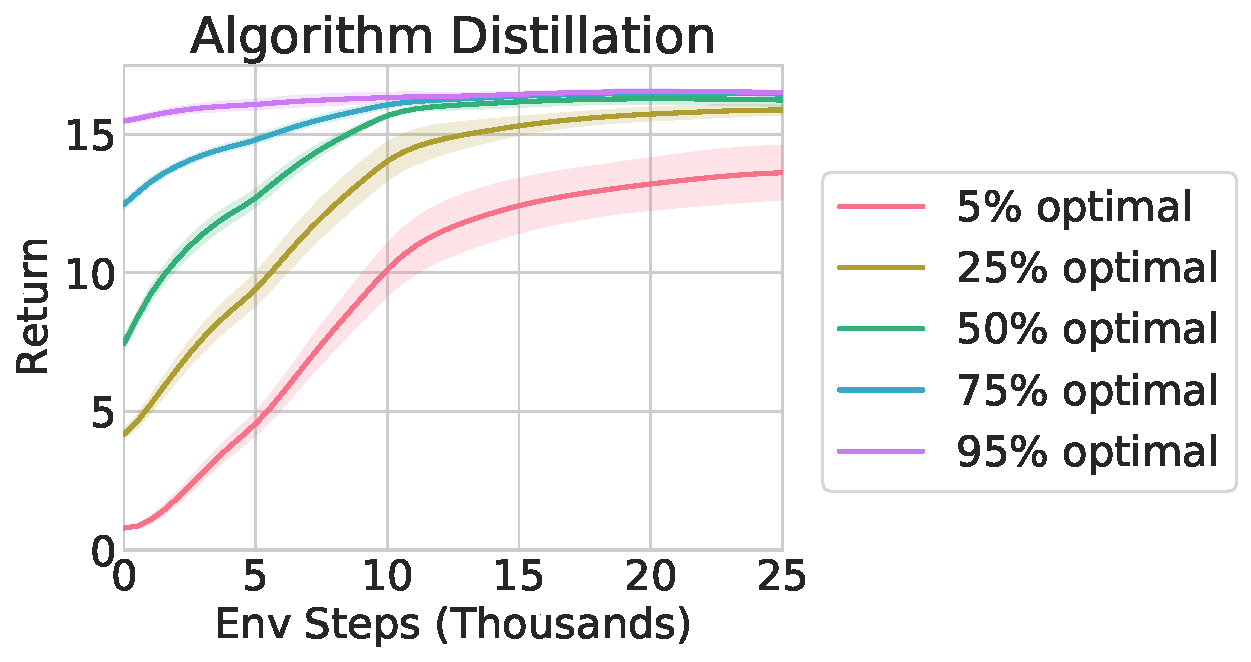
\includegraphics[width=\textwidth]{assets/images/ad_partial_demos.pdf}
    \label{fig:ad_demo}
\end{subfigure}
\hfill
\begin{subfigure}{0.4\textwidth}
    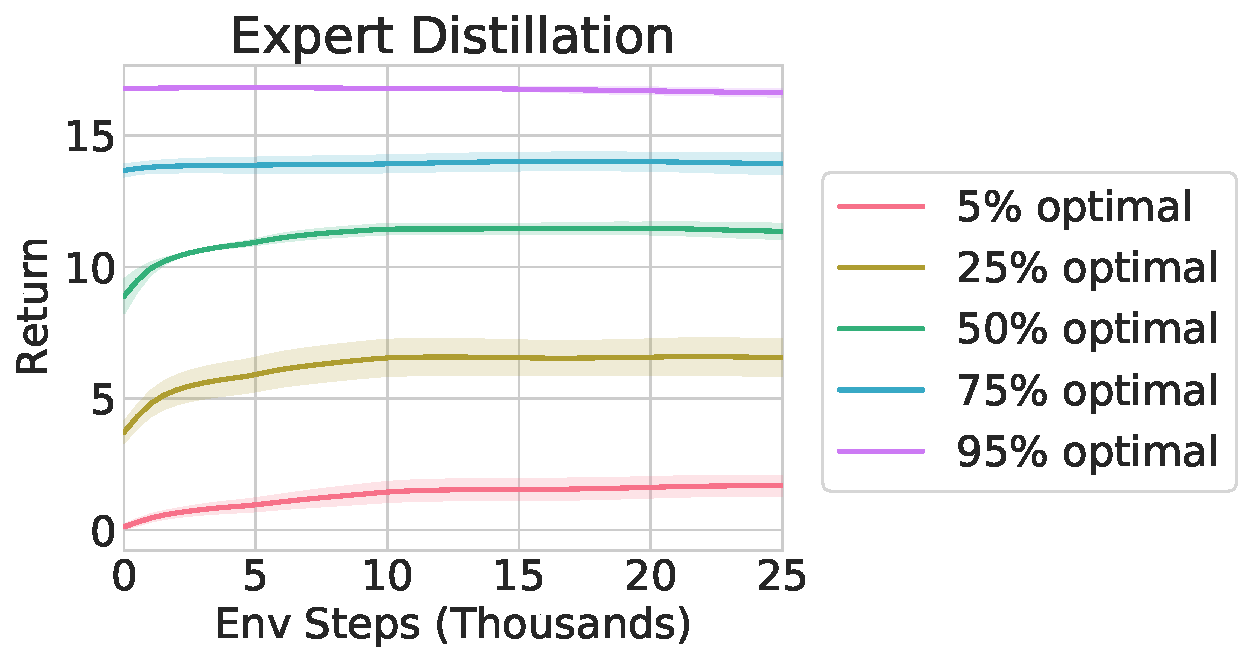
\includegraphics[width=\textwidth]{assets/images/ed_partial_demos.pdf}
    \label{fig:ed_demo}
\end{subfigure}
  \hspace*{\fill}%

\caption{\small {\it AD and ED conditioned on partial demonstrations:} We compare the performance of \name and ED when prompted with a demonstration from the source algorithm's training history on Dark Room (semi-dense). While ED slightly improves and then maintains performance from the input policy, \name is able to improve it in-context until the policy is optimal or nearly optimal. }
\label{fig:ad_ed_cond}
\vspace{-4mm}
\end{figure}

\vspace{-2mm}

\paragraph{Can \fullname learn from pixel-based observations?}
\begin{wrapfigure}{r}{0.4\textwidth}
  \begin{center}
    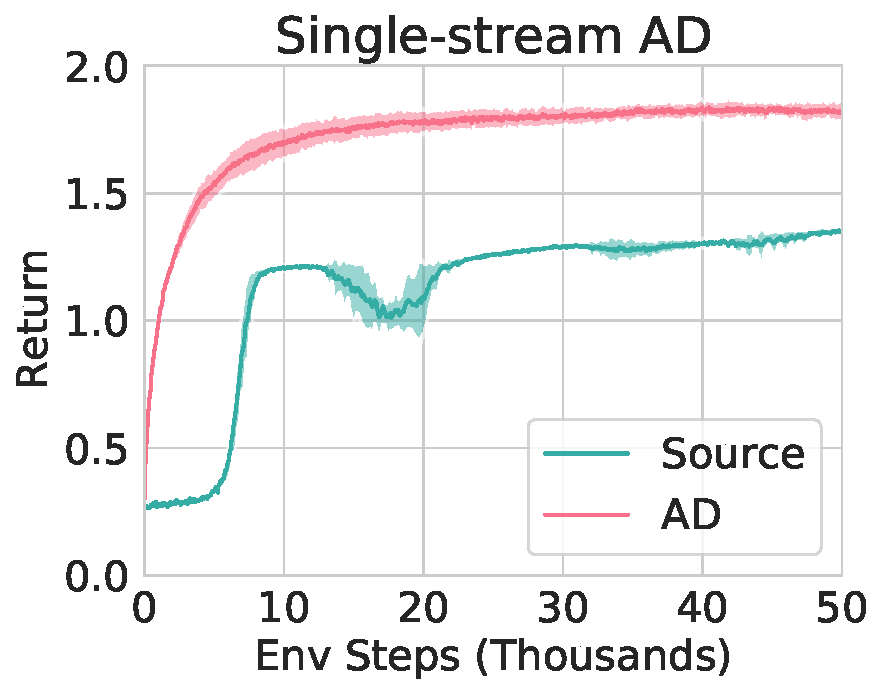
\includegraphics[width=0.3\textwidth]{assets/images/source_algo_comparison.pdf}
  \end{center}
  \caption{\small {\it Single-stream \fullnamenospace:} \name trained on the learning history from an A3C agent with only one actor ({\it i.e.} single-stream). By training on subsampled learning histories (see Sec.~\ref{sec:exps}), \name learns are more data-efficient in-context RL algorithm.}
  \vspace{5mm}
  \label{fig:single_stream_ad}

\end{wrapfigure}
DMLab Watermaze is a pixel-based environment that is larger than the Dark environments with tasks sampled from a continuous uniform distribution. The environment is partially observable in two ways - the goal is invisible until the agent has reached it and the first-person view limits the agent's field of vision. Shown in Fig.~\ref{fig:main_exps}, \name maximizes the episodic return with in-context RL while ED does not learn.

\vspace{-4mm}
\begin{wrapfigure}{r}{0.4\textwidth}
 \vspace{-2mm}
  \begin{center}
    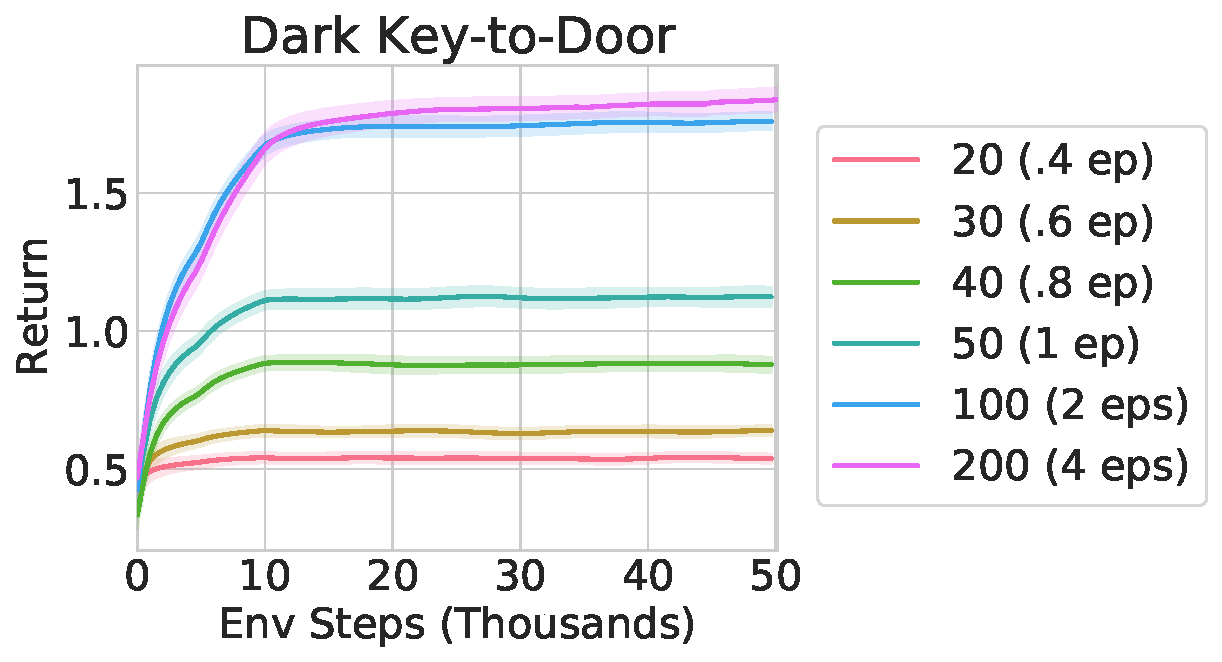
\includegraphics[width=0.39\textwidth]{assets/images/context_size_2g.pdf}
  \end{center}
  \caption{\small {\it Context size:} \name in Dark Key-to-Door with different context sizes. In-context RL only emerges once the context size is large enough and across-episodic.}
  \label{fig:context_size}

\end{wrapfigure}
\paragraph{Can AD learn a more data-efficient RL algorithm than the one that produced the source data?} In Fig.~\ref{fig:main_exps}, \name is significantly more data-efficient than the source algorithm. This gain is a byproduct of distilling a multi-stream algorithm into a single-stream one. The source algorithms (A3C and DQN) are distributed, which means they run many actors in parallel to achieve good performance.\footnote{Indeed, current state-of-the-art RL algorithms such as MuZero~\citep{sch19muzero} and Muesli~\citep{hessel21muesli} rely on distributed actors.}  A distributed RL algorithm may not be very data-efficient in aggregate but each individual actor can be data-efficient. Since the learning history for each actor is saved separately, \name achieves similar performance to the multi-stream distributed RL algorithm, but is more data-efficient as a single-stream method.


These data-efficiency gains are also evident for distilling single-stream algorithms.
In Fig~\ref{fig:single_stream_ad} we show that by subsampling every $k$-th episode (where $k=10$) from a single stream A3C learning history, \name can still learn a more data-efficient in-context RL algorithm (for more detail, see Appendix~\ref{app:single_stream}). Therefore, \name can be more data-efficient than both a multi and single-stream source RL algorithm.

While \name is more data-efficient, the source algorithm achieves slightly higher asymptotic performance (see Appendix~\ref{app:source}). However, the source algorithm produces many single-task agents with a unique set of weights $\phi_n$ per task $\mathcal M_n$, while \name produces a single generalist agent with weights $\theta$ that are fixed across all tasks.


\vspace{-2mm}
\paragraph{Is it possible to accelerate AD by prompting it with demonstrations?}


Although \name can reinforcement learn without relying on demonstrations, it has the added benefit that, unlike the source algorithm, it can be conditioned on or prompted with external data.
To answer the research question, we sample policies from the hold-out test-set data along different points of the source algorithm history - from a near-random policy to a near-expert policy. We then pre-fill the context for both \name and ED with this policy data, and run both methods in the environment in Dark Room  and plot the results in Fig.~\ref{fig:ad_ed_cond}.
While ED maintains the performance of the input policy, \name improves every policy in-context until it is near-optimal. Importantly, the more optimal the input policy the faster \name improves it until it is optimal.






\vspace{-2mm}

\paragraph{What context size is required for in-context RL to emerge?}
We've hypothesized that \name requires sufficiently long (\ie \ across-episodic) contexts to in-context reinforcement learn. We test this hypothesis by training several \name variants with different context sizes on the Dark Room environment. We plot the learning curves of these different variants in Fig.~\ref{fig:context_size} and find that multi-episodic contexts of 2-4 episodes are necessary to learn a near-optimal in-context RL algorithm. Initial signs of in-context RL begin to emerge when the context size is roughly the length of an episode. The reason for this is likely that the context is large enough to retrain across-episodic information -- \eg, at the start of a new episode, the context will be filled with transitions from most of the previous episode.
\looseness=-1

